\chapter{Teoretyczne rozwiązanie problemu}
\thispagestyle{chapterBeginStyle}

Ten rozdział ma za zadanie przedstawić teoretyczną (matematyczną) część rozwiązania głównego problemu -- uzyskania pozycji rzutki. Na początku zaprezentowany i podzielony na części został ogólny pomysł rozwiązania. Pokazane zostały również alternatywne propozycje podejścia do problemu, wraz z uzasadnieniem, dlaczego nie zostały one wybrane. Następnie omówiono podstawowe terminy i zagadnienia, których znajomość potrzebna jest do pełnego zrozumienia dalszych tematów. Główną częścią rozdziału jest prezentacja wszystkich kluczowych obliczeń i operacji, które zachodzą podczas analizy rzutu, krok po kroku. Detale dotyczące niektórych algorytmów zostaną przedstawione w późniejszych rozdziałach, w tym zaś uznaje się je za tzw. czarne skrzynki (ang. \textit{black box}), to znaczy elementy programu, które przyjmują pewne dane wejściowe i zwracają wyniki, lecz ich implementacja nie jest rozważana.

\section{Idea rozwiązania}
Pierwszą decyzją, jaką należało podjąć podczas tworzenia rozwiązania, było ustalenie, na podstawie jakich danych wejściowych system powinien rozpoznawać rzut. Postawiono na ten sam typ danych, którym człowiek posługuje się przy ocenie rzutu, czyli obraz. W systemie rolę wzroku pełnią kamery, które co określony czas dostarczają zdjęcia tarczy. Dzięki ciągłemu porównywaniu następujących po sobie klatek, system wykrywa rzut i rozpoczyna przetwarzanie obrazu z wbitą lotką. Do określenia dokładnej pozycji rzutki wykorzystano metodę triangulacji. Pozwala ona na obliczenie dystansu do obiektu za pomocą zdjęć z dwóch kamer. Tarcza i kamery są zamocowane w stelażu o znanych wymiarach. Kamery w ustalonej odległości od siebie, a ich soczewki są ustawione prostopadle do powierzchni tarczy. Następnie, po zmianie układu współrzędnych, dzięki znanym dokładnym wymiarom tarczy, pozycja rzutki jest przyporządkowywana do konkretnego segmentu punktowego.

Pomysłem również opartym na przetwarzaniu obrazu, jest próba uzyskania miejsca wbicia rzutki z użyciem tylko jednej kamery, która jest umiejscowiona przed tarczą, naprzeciw jej. Obniżyłoby to koszty i ułatwiło obliczenia, jednak byłoby niepraktyczne, ponieważ to gracz musi stać na wprost tarczy, a kamera znajdowałaby się pomiędzy nim a tarczą, w środku strefy lotu. Cechowałoby się to także małą przenoszalnością, trudno byłoby zawsze ustawić kamerę idealnie na wysokości środka tarczy. Gdyby jednak kamera była przesunięta względem półprostej prostopadłej do płaszczyzny tarczy, przechodzącej przez jej środek, to przetwarzanie obrazu i obliczenia mocno by się utrudniły, gdyż kamera patrzyłaby pod pewnym kątem na tarczę. Trudniejsze byłoby również mocowanie kamery.

Kolejnym wariantem, branym pod uwagę przy nakreślaniu rozwiązania, było zastosowanie techniki multilateracji, która polega na określaniu położenia obiektu za pomocą mierzenia różnic w czasie dotarcia sygnału do kilku odbiorników. W omawianym przypadku można by użyć mikrofonów na obrzeżach tarczy, które oczekiwałyby na dźwięk wydany przez wbicie się rzutki. Następnie porównując różnice w czasie wykrycia dźwięku, system mógłby wyliczyć pozycję rzutki. To rozwiązanie również obniżyłoby koszty systemu, lecz dawałoby gorsze rezultaty. Tego typu techniki są przede wszystkim stosowane w geodezji, przy dużych odległościach między odbiornikami a emiterem. Tutaj różnice pomiędzy przybyciem dźwięku do poszczególnych mikrofonów byłyby minimalne, przez co trudne byłoby zachowanie wystarczającej precyzji. Wąskim gardłem byłby również przetwornik analogowo-cyfrowy, ponieważ różnice te mogłyby być mniejsze od różnicy w czasie pomiędzy dwiema kolejnymi próbkami, powstałymi podczas procesu próbkowania w przetworniku.

Pod uwagę brano również analizę obrazu z użyciem sztucznej inteligencji. Potencjalnie można by wytrenować sieć neuronową na podstawie wielu zdjęć tarczy z wbitą rzutką. Najważniejszymi wadami tego rozwiązania w stosunku do metody triangulacji są ograniczone możliwości poprawy w przypadku niezadowalających wyników oraz trudność debugowania. Zaimplementowany ostatecznie sposób można było dużo łatwiej podzielić na części, sprawdzić małe elementy systemu, dzięki czemu błędy w działaniu programu są szybciej lokalizowane i naprawiane. W każdym momencie autor kodu źródłowego jest świadomy, jakie procesy zachodzą w systemie i może na nie wpływać, ograniczona jest rola tzw. czarnych skrzynek. Prawdopodobnie, gdyby użyto sztucznej inteligencji, niemożliwe byłoby uzyskanie np. pozycji rzutki we współrzędnych kartezjańskich, a jedyną daną wyjściową byłoby pole, w jaki trafiła lotka.

\section{Podstawy fotografii}
Urządzeniem, które jest w stanie dostarczać optyczne odzwierciedlenia ograniczonego wycinka przestrzeni trójwymiarowej za pomocą dwuwymiarowych zdjęć, jest aparat fotograficzny. Z biegiem czasu stawał się on coraz bardziej zaawansowany technologicznie, jednak do potrzeb niniejszej pracy wystarczającym modelem jest pierwszy model aparatu, czyli aparat otworkowy (\textit{camera obscura}). Jego budowa jest bardzo prosta: w zaciemnionym pudełku, na jednej z jego ścian tworzy się niewielki otwór, za pomocą którego wpada światło. Na przeciwległej ścianie tworzy się obrócony obraz tego, co znajduje się na wprost pudełka. Schemat działania aparatu otworkowego pokazany jest na rysunku \ref{camera_obscura}.

\begin{figure}[h!]
\begin{center}
\includesvg[width=0.5\textwidth]{obrazki/pinhole_camera.svg}
\end{center}
\captionsource{{\color{dgray}Zasada działania aparatu otworkowego}}{http://commons.wikimedia.org/wiki/Image:Pinhole-camera.png}
\label{camera_obscura}
\end{figure} 

W schematach (zwłaszcza związanych z grafiką komputerową) często przedstawia się powyższy model w uproszczonej formie, gdzie obraz tworzy się pomiędzy środkiem aparatu (otworem) a fotografowanym obiektem \cite{Pinhole_MSc}. Przykład takiego schematu jest widoczny na rysunku \ref{pinhole_model}. Osie $XYZ$ reprezentują trójwymiarowy układ współrzędnych, którego początkiem jest środek aparatu, oznaczony jako $C$. W tym samym układzie jest fotografowany obiekt (punkt), zaznaczony literą $P$. W odległości $f$ od środka kamery, zwanej jako ogniskowa, znajduje się fragment płaszczyzny, nazywanej płaszczyzną obrazu (eng. \textit{image plane}), na której powstaje obraz. Oś $Z$ jest do niej prostopadła i przechodzi przez jej środek. Z płaszczyzną związany jest dwuwymiarowy układ współrzędnych. Odzwierciedleniem punktu $P$ na obrazie jest punkt $P'$. Powstaje on na skutek przecięcia się półprostej (eng. \textit{ray}, na rysunku jako $r$) przechodzącej przez środek kamery i punkt $P$ z płaszczyzną obrazu. Jest to analogia do pojedynczego promienia światła, które wpada przez otwór w aparacie otworkowym. Ponieważ trójwymiarowe punkty są przedstawiane w dwuwymiarowym układzie, tracimy informacje o głębokości, a punkt na obrazie reprezentuje nieskończoną liczbę punktów znajdujących się na prostej $r$.

\begin{figure}[h!]
\begin{center}
\includesvg[width=0.5\textwidth]{obrazki/pinhole_model.svg}
\end{center}
\captionsource{{\color{dgray}Diagram optyczny aparatu otworkowego}}{Opracowanie własne}
\label{pinhole_model}
\end{figure} 

W systemie zostały użyte kamery, dzięki którym można zaobserwować ruch. Ich fizyczna budowa nie różni się od aparatu, są one jedynie przystosowane do tego, by robić wiele zdjęć w krótkim czasie, dzięki czemu, po wyświetleniu zdjęć jeden po drugim, mózg interpretuje je jako ciągły ruch.

Przed przedłożeniem całego procesu przetwarzania i analizy obrazu, należy zrozumieć, czym jest obraz z informatycznego punktu widzenia. Zdjęcie cyfrowe (w grafice rastrowej) interpretowane jest jako macierz $A_{m \times n} = [a_{ij}]$, gdzie każdy element $a_{ij}$ odpowiada jednemu pikselowi, czyli kwadratowi wypełnionemu jednolitym kolorem. Piksele powstają z podzielenia płaszczyzny obrazu na gęstą siatkę niewielkich kwadratów. Kolor piksela najczęściej reprezentowany jest jako trójka uporządkowana $(r, g, b)$, gdzie $r$ oznacza intensywność koloru czerwonego, $g$ -- zielonego, a $b$ -- niebieskiego. Standardowo, każda z trzech składowych koloru jest zapisywana na 8 bitach i przyjmuje wartości od 0 do 255. Złożenie na siebie tych trzech barw podstawowych w różnym stopniu nasycenia pozwala na przedstawianie dowolnej barwy.
% TODO, można dodać grafikę w stylu: obraz 3x3 -> macierz z RGB

\section{Triangulacja}
Pojęcie triangulacji jest różnie rozumiane w zależności od okoliczności, w jakich jest używane. W geometrii (podobnie jak w grafice komputerowej) oznacza ono proces podziału figury na trójkąty, w socjologii metodę prowadzenia badań społecznych, zaś w teorii grafów triangulacją grafu $G$ można nazywać maksymalny planarny nadgraf grafu $G$. Należy zatem jasno podkreślić, w jaki sposób rozumiany jest ten termin w niniejszej pracy. Wiąże się on z dwoma dziedzinami: geodezją i rozpoznawaniem obrazów (lub widzeniem komputerowym, od ang. \textit{computer vision}). W obu przypadkach oznacza on wyznaczenie pozycji lub odległości do obiektu za pomocą danych z dwóch miejsc, pomiędzy którymi dystans jest znany.

Triangulacja w geodezji jest używana od wielu lat, dzięki niej uzyskano przybliżone wymiary Ziemi oraz skonstruowano wiele map.
Znając położenie punktów $A$ i $B$, możliwe jest uzyskanie pozycji punktu $C$, widocznego z $A$ i $B$. W tym celu, oblicza się kąty $\measuredangle CAB$ z punktu $A$ i $\measuredangle CBA$ z punktu $B$. Następnie, konstruuje się trójkąt $ABC$. Znając długość odcinka $|AB|$ i oba kąty z nim sąsiadujące, możliwe jest jednoznaczne wyznaczenie wszystkich boków trójkąta, dzięki czemu uzyskuje się odległość do mierzonego obiektu. Dzięki powtarzaniu tej metody, gdzie nowo zmierzony punkt staje się daną wejściową do kolejnego pomiaru, możliwe jest tworzenie całych sieci triangulacyjnych, np. pomiędzy miastami.
% TODO: można prosty obrazek trójkąta

Rozpoznawanie obrazów interpretuje triangulację bezpośrednio w odniesieniu do zdjęć. Do wytłumaczenia pojęcia w tym kontekście często używa się geometrii epipolarnej (wielobiegunowej). Polega ona na umieszczeniu dwóch modeli z rysunku \ref{pinhole_model} w jednym układzie. Typowy, prosty model tej geometrii, przedstawiono na rysunku \ref{epipolar}. Widać na nim dwa aparaty (model otworkowy), ustawione pod kątem 45 stopni do czytelnika, gdzie kąt pomiędzy jednym a drugim aparatem wynosi 90 stopni. Na podstawie danych z jednej kamery można uzyskać informację o półprostej przechodzącej przez szukany punkt. Dwie kamery dają dwie takie półproste, których miejsce przecięcia określi jednoznacznie położenie obiektu. Niestety, w rzeczywistości wiele etapów powstawania i przetwarzania obrazu jest narażone na błędy, przez co półproste w praktyce nigdy nie będą idealnie odzwierciedlać rzeczywistości. Wpływają na to zniekształcenia wprowadzane przez soczewkę optyczną, błędy pomiarów odległości między kamerami czy zaawansowanie technologiczne kamer (nie są one zgodne z modelem otworkowym, a także zawierają np. oprogramowanie sprzętowe zmieniające zdjęcie w celu jego poprawy). Powoduje to jednak nie tylko zmniejszenie dokładności, ale sytuację, gdzie przeprowadzenie triangulacji nie będzie w ogóle możliwe, gdyż półproste mogą się nie przeciąć, przez co nie uda się uzyskać pożądanego punktu. Wprowadza to konieczność przetwarzania półprostych w takim celu, by zminimalizować błąd i znaleźć najlepsze przybliżenie szukanego punktu. Stosuje się w tym celu różne metody, których opis przekracza zakres tej pracy.

\begin{figure}[h!]
\begin{center}
\includesvg[width=0.5\textwidth]{obrazki/epipolar.svg}
\end{center}
\captionsource{{\color{dgray}Geometria epipolarna}}{Opracowanie własne}
\label{epipolar}
\end{figure} 

Metoda triangulacji zaimplementowana w obecnej wersji systemu jest połączeniem obu metod. Działa ona w oparciu o dwie kamery skierowane do siebie pod kątem prostym i analizuje dwuwymiarowe obrazy przez nie dostarczone, przetwarza współrzędne pikseli. Różni się ona jednak od klasycznego podejścia do triangulacji, używanego w widzeniu komputerowym: zamiast wyznaczania półprostych ze środka kamery, przechodzących przez punkt na obrazie, a następnie prób wyznaczenia przecięcia tychże półprostych, wyznaczane i poddane obliczeniom są przybliżone kąty dla każdej z kamer, analogicznie jak w wyżej przedstawionym, geodezyjnym podejściu do problemu. Początkowo planowano zaimplementowanie tej wersji jedynie jako pierwsze przybliżenie pozycji rzutki z powodu mniejszej liczby dodatkowych problemów do rozwiązania, ale okazała się ona na tyle dokładna, że pozostawiono ją. Jest to jednak pole do dalszych badań, mogących podnieść skuteczność systemu.

\section{Stelaż}
W systemie, w którym dokładność ma tak duże znaczenie, podczas każdego etapu projektowania i implementacji, należy pamiętać o zminimalizowaniu ewentualnych błędów. Stąd wynika konieczność stabilizacji układu tarcza-kamera-kamera, tak by wszystkie wymiary konieczne do przeprowadzenia triangulacji były ustalone i nie zmieniały się pomiędzy poszczególnymi testami. 

Częścią, która spełnia te potrzeby, jest stelaż wykonany z drewna. Ma on kształt niskiego, otwartego prostopadłościanu (bez jednej ściany). W jego lewym górnym rogu umiejscowiona jest tarcza. Jedna kamera znajduje się na prawym (patrząc z góry) boku prostopadłościanu, na linii poziomej, przechodzącej przez środek tarczy, druga zaś na dolnym boku, na linii pionowej. Schematyczny rzut z góry na stelaż pokazany jest na rysunku \ref{stelaz_gora}, a zdjęcie wykonanego stelaża na rysunku \ref{stelaz_zdjecie}.

\begin{figure}[h!]
\centering
\begin{subfigure}{\textwidth}
  \centering
  \includesvg[width=0.5\textwidth]{obrazki/stelaz_mockup.svg}
  \captionsource{{\color{dgray}Szkic stelażu (rzut z góry)}}{Opracowanie własne}
  \label{stelaz_gora}
\end{subfigure}
\begin{subfigure}{\textwidth}
  \vspace{1cm}
  \centering
  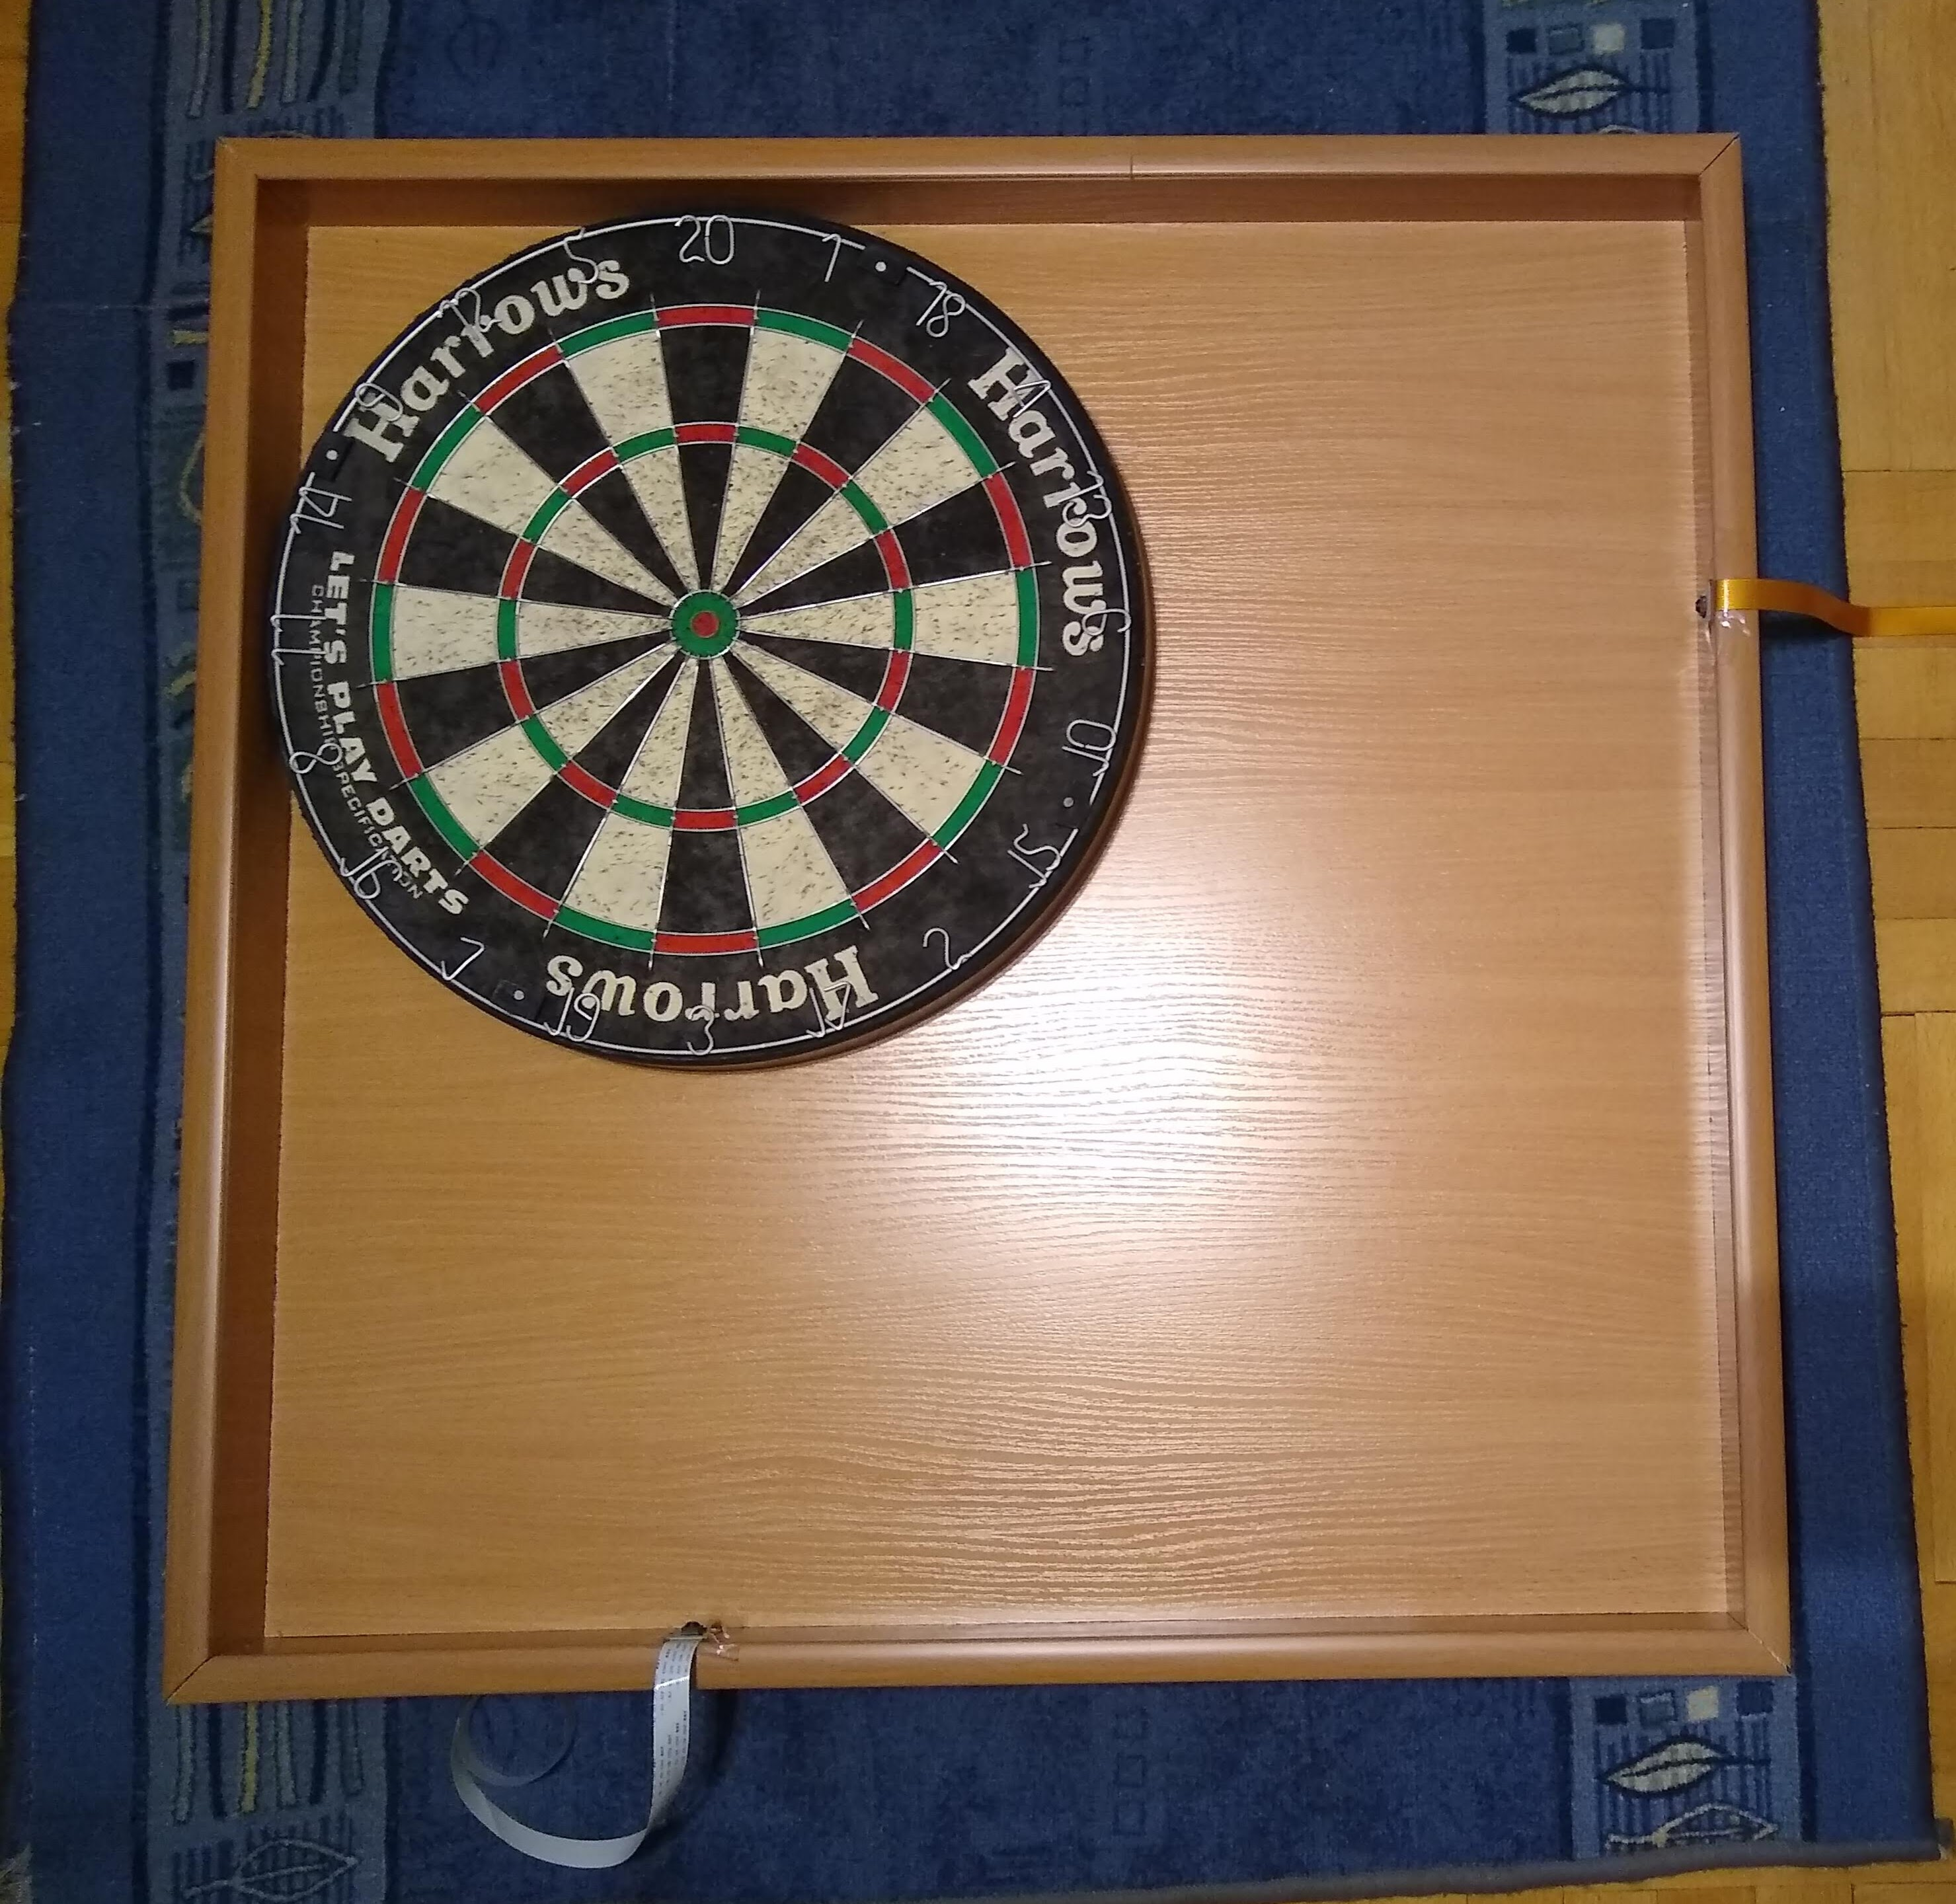
\includegraphics[width=0.5\textwidth]{obrazki/stelaz_live.jpg}
  \captionsource{{\color{dgray}Ukończony stelaż}}{Opracowanie własne}
  \label{stelaz_zdjecie}
\end{subfigure}
\end{figure}

Przed wykonaniem stelaża należało określić, jakie powinien mieć wymiary. Podstawowym warunkiem było to, że kamera musi obejmować cały obszar tarczy, a jednocześnie cały stelaż powinien być jak najmniejszy. Dlatego pierwszym krokiem było odpowiedzenie na pytanie:

\begin{question}
W jakiej minimalnej odległości od środka tarczy w kształcie koła o promieniu $r$ powinna znaleźć się kamera o kącie widzenia $\alpha$, by na zdjęciu cała tarcza była widoczna? 
\end{question}

\begin{figure}[h!]
\begin{center}
\includesvg[width=0.5\textwidth]{obrazki/odleglosc_kamery.svg}
\end{center}
\captionsource{{\color{dgray}Rysunek pomocniczy}}{Opracowanie własne}
\label{odleglosc_kamery}
\end{figure} 

Do przedstawienia rozwiązania pomocny jest rysunek \ref{odleglosc_kamery}. $P$ oznacza środek kamery, $O$ to środek tarczy (początek układu współrzędnych), $d$ to odległość pomiędzy $P$ a $O$. Przyjmuje się, że kamera jest zwrócona dokładnie na wprost tarczy, dlatego odcinek $OP$ jest dwusieczną kąta $APB$. Pole wyznaczone przez półproste $l$ i $m$ to pole widzenia kamery. By cała tarcza była widoczna, koło musi być zawarte w tym polu. Ponieważ zadaniem jest znalezienie minimalnej odległości, wystarczy by proste $l$ i $m$ były styczne do okręgu. \newline

\noindent Kąty:
\begin{gather*}
\measuredangle PAO = \measuredangle PBO = \pi - \frac{\pi}{2} - \frac{\alpha}{2} = \frac{\pi - \alpha}{2} 
\end{gather*}
Równania prostych i okręgu:
\begin{gather*}
l: y = a_1x + b_1 \\
m: y = a_2x + b_2 \\
x^2 + y^2 = r^2
\end{gather*}
Ponieważ współczynnik kierunkowy prostej jest równy tangensowi kąta nachylenia do osi $OX$, otrzymuje się:
\begin{gather*}
a_1 = \tan (\frac{\pi - \alpha}{2}) \\ 
a_2 = \tan (\pi - \frac{\pi - \alpha}{2}) = \tan (\frac{\pi + \alpha}{2})
\end{gather*}
Półproste $l$ i $m$ przecinają się w punkcie $P(0, d)$:
\begin{gather*}
a_1 \cdot 0 + b_1 = a_2 \cdot 0 + b_2 \\
b_1 = b_2 = d
\end{gather*}
Proste przecinają się z osią $OY$ w tym samym punkcie, więc mają ten sam wyraz wolny, równy $d$.
\begin{gather*}
l: y = \tan (\frac{\pi - \alpha}{2})x + d \\
m: y = \tan (\frac{\pi + \alpha}{2})x + d
\end{gather*}
Teraz wystarczy, by następujący układ równań miał jedno rozwiązanie (można by również użyć równania drugiej prostej, nie ma to znaczenia):
\begin{gather*}
x^2 + y^2 = r^2 \\ 
y = \tan (\frac{\pi + \alpha}{2})x + d
\end{gather*}
Podstawienie:
\begin{gather*}
x^2 + (\tan(\frac{\pi + \alpha}{2})x + d)^2 - r^2 = 0 \\
x^2 + \tan^2(\frac{\pi + \alpha}{2})x^2 + 2\tan(\frac{\pi + \alpha}{2})dx + d^2 - r^2 = 0 \\
[\tan^2(\frac{\pi + \alpha}{2}) + 1]x^2 + 2\tan(\frac{\pi + \alpha}{2})dx + d^2 - r^2 = 0
\end{gather*}
To równanie kwadratowe musi mieć dokładnie jedno rozwiązanie, dlatego $\Delta = 0$:
\begin{equation*}
\begin{split}
\Delta & = [2\tan(\frac{\pi + \alpha}{2})d]^2 - 4\cdot[\tan^2(\frac{\pi + \alpha}{2}) + 1]\cdot (d^2 - r^2) = \\
 & = 4\tan^2(\frac{\pi + \alpha}{2})d^2 - 4[\tan^2(\frac{\pi + \alpha}{2})d^2 - \tan^2(\frac{\pi + \alpha}{2})r^2 + d^2 - r^2] = \\
 & = 4[\tan^2(\frac{\pi + \alpha}{2})d^2 - \tan^2(\frac{\pi + \alpha}{2})d^2 + \tan^2(\frac{\pi + \alpha}{2})r^2 - d^2 + r^2] = \\
 & = 4[(\tan^2(\frac{\pi + \alpha}{2}) + 1)r^2 - d^2]
\end{split}
\end{equation*}
\begin{gather*}
\Delta = 0 \\
4[(\tan^2(\frac{\pi + \alpha}{2}) + 1)r^2 - d^2] = 0 \\
(\tan^2(\frac{\pi + \alpha}{2}) + 1)r^2 - d^2 = 0 \\
d^2 = (\tan^2(\frac{\pi + \alpha}{2}) + 1)r^2 \\
d_1 = r\sqrt{\tan^2(\frac{\pi + \alpha}{2}) + 1} \lor d_2 = - r\sqrt{\tan^2(\frac{\pi + \alpha}{2}) + 1}
\end{gather*}
Ponieważ $d > 0$ (z rysunku), to można odrzucić rozwiązanie $d_2$ -- wyrażenie pod pierwiastkiem jest dodatnie (kwadrat zwiększony o jeden), promień również jest dodatni, więc całe $d_2 < 0$. Ostatecznie:
\begin{gather*}
d = r\sqrt{\tan^2(\frac{\pi + \alpha}{2}) + 1}
\end{gather*}
Dla tarczy i kamery użytych w systemie, gdzie $r = 22,5$ cm, a $\alpha = 53,37\degree$, $d = 50,1$ cm.

Na podstawie tej wartości ustalono wymiary całego stelaża. Najmniejsze możliwe wymiary, to $(d + r) \times (d + r)$, czyli $72,6$ cm $\times \ 72,6$ cm. Wykonany stelaż jest nieco większy ($74,5$ cm $\times \ 74,5$ cm), m.in. z powodu uwzględnienia niezerowej grubości kamery oraz pozostawienia zapasu na ewentualne modyfikacje i pomyłki.
% TODO: można dodać info o trzecim wymiarze (wysokości), zarówno w rysunkach, jak i obliczeniach

\begin{gather*}
\end{gather*}
